

\tikzset{every picture/.style={line width=0.75pt}} %set default line width to 0.75pt        

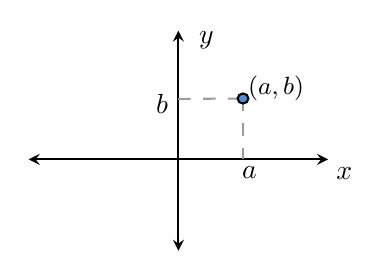
\begin{tikzpicture}[x=0.75pt,y=0.75pt,yscale=-1,xscale=1, scale=0.4]
%uncomment if require: \path (0,300); %set diagram left start at 0, and has height of 300

%Straight Lines [id:da31875425075049346] 
\draw[stealth-stealth](331.3,13.87) -- (331.3,279) ;

%Straight Lines [id:da7321937935224139] 
\draw[stealth-stealth](151,168.96) -- (511.61,168.96) ;

%Straight Lines [id:da914186055379401] 
\draw [color={rgb, 255:red, 155; green, 155; blue, 155 }  ,draw opacity=1 ] [dash pattern={on 4.5pt off 4.5pt}]  (409.14,95.65) -- (409.14,168.72) ;
%Straight Lines [id:da11993693614621659] 
\draw [color={rgb, 255:red, 155; green, 155; blue, 155 }  ,draw opacity=1 ] [dash pattern={on 4.5pt off 4.5pt}]  (331.04,96.14) -- (409.14,95.65) ;
%Shape: Ellipse [id:dp09496336303029529] 
\draw  [fill={rgb, 255:red, 74; green, 144; blue, 226 }  ,fill opacity=1 ] (402.67,95.65) .. controls (402.67,92.29) and (405.57,89.57) .. (409.14,89.57) .. controls (412.71,89.57) and (415.6,92.29) .. (415.6,95.65) .. controls (415.6,99.02) and (412.71,101.74) .. (409.14,101.74) .. controls (405.57,101.74) and (402.67,99.02) .. (402.67,95.65) -- cycle ;

% Text Node
\draw (517.95,174.76) node [anchor=north west][inner sep=0.75pt]    {$x$};
% Text Node
\draw (352.45,11.58) node [anchor=north west][inner sep=0.75pt]    {$y$};
% Text Node
\draw (411.64,64.21) node [anchor=north west][inner sep=0.75pt]  [font=\small]  {$( a,b)$};
% Text Node
\draw (404.17,173.54) node [anchor=north west][inner sep=0.75pt]    {$a$};
% Text Node
\draw (300.67,86.47) node [anchor=north west][inner sep=0.75pt]    {$b$};


\end{tikzpicture}
